\subsection{Identifying Component 3 in Figure T-1}
\label{T6C04}

\begin{tcolorbox}[colback=gray!10!white,colframe=black!75!black,title=T6C04]
What is component 3 in figure T-1?

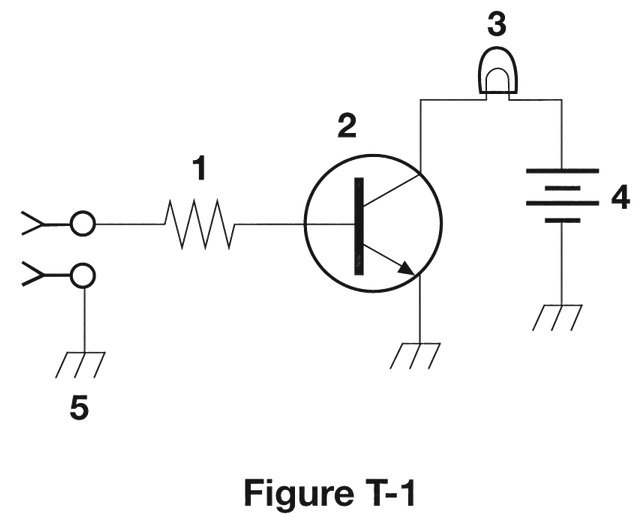
\includegraphics[width=0.5\textwidth]{tech/images/t1.png} 



\begin{enumerate}[label=\Alph*)]
    \item Resistor
    \item Transistor
    \item \textbf{Lamp}
    \item Ground symbol
\end{enumerate}
\end{tcolorbox}

\subsubsection{Intuitive Explanation}
Imagine you’re looking at a picture of a simple circuit, like a flashlight. In this picture, there’s a part that lights up when you turn it on. That’s the lamp! It’s like the bulb in your flashlight that glows when you press the button. So, if someone asks you, “What’s the part that lights up?” you’d say, “That’s the lamp!” Easy, right?

\subsubsection{Advanced Explanation}
In the context of electrical circuits, a lamp is a component that converts electrical energy into light energy. It typically consists of a filament that heats up and emits light when current passes through it. In schematic diagrams, a lamp is often represented by a specific symbol that resembles a circle with a cross inside it. 

To identify component 3 in figure T-1, you would look for this symbol. The lamp is distinct from other components like resistors, which limit current flow, transistors, which amplify or switch electronic signals, and ground symbols, which represent the reference point in a circuit. 

Understanding the symbols used in schematic diagrams is crucial for interpreting and designing electronic circuits. Each component has a unique symbol that helps engineers and technicians quickly identify its function within the circuit.

% Prompt for generating the diagram:
% Include a diagram of figure T-1 with component 3 clearly labeled as a lamp. The diagram should show the lamp symbol in the context of a simple circuit.